
\documentclass[letterpaper,hide notes,xcolor={table,svgnames},pdftex,10pt]{beamer}
\def\showexamples{t}

\usecolortheme{crane}
\setbeamertemplate{navigation symbols}{}

\usetheme{MyPittsburgh}
\usepackage{hyperref}
\usepackage{graphicx,xspace}
\usepackage[normalem]{ulem}
\usepackage{multicol}
\usepackage{amsmath,amssymb,amsthm,graphicx,xspace}
\newcommand\SF[1]{$\bigstar$\footnote{SF: #1}}

\usepackage[sfdefault,lf]{carlito}
\usepackage[T1]{fontenc}
\usepackage[scaled]{beramono}
\usepackage{tikzpagenodes}
\newcommand{\Rplus}{\protect\hspace{-.1em}\protect\raisebox{.35ex}{\small{\small\textbf{+}}}}
\newcommand{\Cpp}{\mbox{C\Rplus\Rplus}\xspace}

\newcounter{tmpnumSlide}
\newcounter{tmpnumNote}

\newcommand\mnote[1]{%
	\addtocounter{tmpnumSlide}{1}
	\ifdefined\showcues {~\tiny\fbox{\arabic{tmpnumSlide}}}\fi
	\note{\setlength{\parskip}{1ex}\addtocounter{tmpnumNote}{1}\textbf{\Large \arabic{tmpnumNote}:} {#1\par}}}

\newcommand\mmnote[1]{\note{\setlength{\parskip}{1ex}#1\par}}


\newcommand\mquestion[2]{{~\color{red}\fbox{?}}\note{\setlength{\parskip}{1ex}\par{\Large \textbf{?}} #1} \note{\setlength{\parskip}{1ex}\par{\Large \textbf{A}} #2\par}\ifdefined \presentationonly \pause \fi}

\newcommand\blackboard[1]{%
	\ifdefined   \showblackboard
		{#1}
	\else {\begin{center} \fbox{\colorbox{blue!30}{%
						\begin{minipage}{.95\linewidth}%
							\hspace{\stretch{1}} Some space intentionally left blank; done at the blackboard.%
						\end{minipage}}}\end{center}}%
	\fi%
}

\usepackage{listings}
\lstset{%
	keywordstyle=\bfseries,
	aboveskip=15pt,
	belowskip=15pt,
	captionpos=b,
	identifierstyle=\ttfamily,
	frame=lines,
	numbers=left, basicstyle=\scriptsize, numberstyle=\tiny, stepnumber=0, numbersep=2pt}

\usepackage{siunitx}
\newcommand\sius[1]{\num[group-separator = {,}]{#1}\si{\micro\second}}
\newcommand\sims[1]{\num[group-separator = {,}]{#1}\si{\milli\second}}
\newcommand\sins[1]{\num[group-separator = {,}]{#1}\si{\nano\second}}
\sisetup{group-separator = {,}, group-digits = true}

%% -------------------- tikz --------------------
\usepackage{tikz}
\usetikzlibrary{positioning}
\usetikzlibrary{arrows,backgrounds,automata,decorations.shapes,decorations.pathmorphing,decorations.markings,decorations.text}

\tikzstyle{place}=[circle,draw=blue!50,fill=blue!20,thick, inner sep=0pt,minimum size=6mm]
\tikzstyle{transition}=[rectangle,draw=black!50,fill=black!20,thick, inner sep=0pt,minimum size=4mm]

\tikzstyle{block}=[rectangle,draw=black, thick, inner sep=5pt]
\tikzstyle{bullet}=[circle,draw=black, fill=black, thin, inner sep=2pt]

\tikzstyle{pre}=[<-,shorten <=1pt,>=stealth',semithick]
\tikzstyle{post}=[->,shorten >=1pt,>=stealth',semithick]
\tikzstyle{bi}=[<->,shorten >=1pt,shorten <=1pt, >=stealth',semithick]

\tikzstyle{mut}=[-,>=stealth',semithick]

\tikzstyle{treereset}=[dashed,->, shorten >=1pt,>=stealth',thin]

\usepackage{ifmtarg}
\usepackage{xifthen}
\makeatletter
% new counter to now which frame it is within the sequence
\newcounter{multiframecounter}
% initialize buffer for previously used frame title
\gdef\lastframetitle{\textit{undefined}}
% new environment for a multi-frame
\newenvironment{multiframe}[1][]{%
	\ifthenelse{\isempty{#1}}{%
		% if no frame title was set via optional parameter,
		% only increase sequence counter by 1
		\addtocounter{multiframecounter}{1}%
	}{%
		% new frame title has been provided, thus
		% reset sequence counter to 1 and buffer frame title for later use
		\setcounter{multiframecounter}{1}%
		\gdef\lastframetitle{#1}%
	}%
	% start conventional frame environment and
	% automatically set frame title followed by sequence counter
	\begin{frame}%
		\frametitle{\lastframetitle~{\normalfont(\arabic{multiframecounter})}}%
		}{%
	\end{frame}%
}
\makeatother

\makeatletter
\newdimen\tu@tmpa%
\newdimen\ydiffl%
\newdimen\xdiffl%
\newcommand\ydiff[2]{%
	\coordinate (tmpnamea) at (#1);%
	\coordinate (tmpnameb) at (#2);%
	\pgfextracty{\tu@tmpa}{\pgfpointanchor{tmpnamea}{center}}%
	\pgfextracty{\ydiffl}{\pgfpointanchor{tmpnameb}{center}}%
	\advance\ydiffl by -\tu@tmpa%
}
\newcommand\xdiff[2]{%
	\coordinate (tmpnamea) at (#1);%
	\coordinate (tmpnameb) at (#2);%
	\pgfextractx{\tu@tmpa}{\pgfpointanchor{tmpnamea}{center}}%
	\pgfextractx{\xdiffl}{\pgfpointanchor{tmpnameb}{center}}%
	\advance\xdiffl by -\tu@tmpa%
}
\makeatother
\newcommand{\copyrightbox}[3][r]{%
	\begin{tikzpicture}%
		\node[inner sep=0pt,minimum size=2em](ciimage){#2};
		\usefont{OT1}{phv}{n}{n}\fontsize{4}{4}\selectfont
		\ydiff{ciimage.south}{ciimage.north}
		\xdiff{ciimage.west}{ciimage.east}
		\ifthenelse{\equal{#1}{r}}{%
			\node[inner sep=0pt,right=1ex of ciimage.south east,anchor=north west,rotate=90]%
			{\raggedleft\color{black!50}\parbox{\the\ydiffl}{\raggedright{}#3}};%
		}{%
			\ifthenelse{\equal{#1}{l}}{%
				\node[inner sep=0pt,right=1ex of ciimage.south west,anchor=south west,rotate=90]%
				{\raggedleft\color{black!50}\parbox{\the\ydiffl}{\raggedright{}#3}};%
			}{%
				\node[inner sep=0pt,below=1ex of ciimage.south west,anchor=north west]%
				{\raggedleft\color{black!50}\parbox{\the\xdiffl}{\raggedright{}#3}};%
			}
		}
	\end{tikzpicture}
}


%% --------------------

%\usepackage[excludeor]{everyhook}
%\PushPreHook{par}{\setbox0=\lastbox\llap{MUH}}\box0}

%\vspace*{\stretch{1}

%\setbox0=\lastbox \llap{\textbullet\enskip}\box0}

\setlength{\parskip}{\fill}

\newcommand\noskips{\setlength{\parskip}{1ex}}
\newcommand\doskips{\setlength{\parskip}{\fill}}

\newcommand\xx{\par\vspace*{\stretch{1}}\par}
\newcommand\xxs{\par\vspace*{2ex}\par}
\newcommand\tuple[1]{\langle #1 \rangle}
\newcommand\code[1]{{\sf \footnotesize #1}}
\newcommand\ex[1]{\uline{Example:} \ifdefined \presentationonly \pause \fi
	\ifdefined\showexamples#1\xspace\else{\uline{\hspace*{2cm}}}\fi}

\newcommand\ceil[1]{\lceil #1 \rceil}


\AtBeginSection[]
{
	\begin{frame}
		\frametitle{Outline}
		\tableofcontents[currentsection]
	\end{frame}
}



\pgfdeclarelayer{edgelayer}
\pgfdeclarelayer{nodelayer}
\pgfsetlayers{edgelayer,nodelayer,main}

\tikzstyle{none}=[inner sep=0pt]
\tikzstyle{rn}=[circle,fill=Red,draw=Black,line width=0.8 pt]
\tikzstyle{gn}=[circle,fill=Lime,draw=Black,line width=0.8 pt]
\tikzstyle{yn}=[circle,fill=Yellow,draw=Black,line width=0.8 pt]
\tikzstyle{empty}=[circle,fill=White,draw=Black]
\tikzstyle{bw} = [rectangle, draw, fill=blue!20,
text width=4em, text centered, rounded corners, minimum height=2em]

\newcommand{\CcNote}[1]{% longname
	This work is licensed under the \textit{Creative Commons #1 3.0 License}.%
}
\newcommand{\CcImageBy}[1]{%
	\includegraphics[scale=#1]{creative_commons/cc_by_30.pdf}%
}
\newcommand{\CcImageSa}[1]{%
	\includegraphics[scale=#1]{creative_commons/cc_sa_30.pdf}%
}
\newcommand{\CcImageNc}[1]{%
	\includegraphics[scale=#1]{creative_commons/cc_nc_30.pdf}%
}
\newcommand{\CcGroupBySa}[2]{% zoom, gap
	\CcImageBy{#1}\hspace*{#2}\CcImageNc{#1}\hspace*{#2}\CcImageSa{#1}%
}
\newcommand{\CcLongnameByNcSa}{Attribution-NonCommercial-ShareAlike}

\newenvironment{changemargin}[1]{% 
	\begin{list}{}{% 
		\setlength{\topsep}{0pt}% 
		\setlength{\leftmargin}{#1}% 
		\setlength{\rightmargin}{1em}
		\setlength{\listparindent}{\parindent}% 
		\setlength{\itemindent}{\parindent}% 
		      \setlength{\parsep}{\parskip}% 
		      }% 
		\item[]}{\end{list}}




\title{Lecture 1 ---Introduction, Operating Systems, Security}

\author{Jeff Zarnett \\ \small \texttt{jzarnett@uwaterloo.ca}}
\institute{Department of Electrical and Computer Engineering \\
  University of Waterloo}
\date{\today}


\begin{document}

\begin{frame}
  \titlepage

 \end{frame}

\begin{frame}
\frametitle{Course Syllabus}

As our first order of business, let's go over the course syllabus.

\end{frame}

\begin{frame}
\frametitle{Collaborative Course}

The source material for the SE~350 notes and slides is open-sourced via Github. 

If you find an error in the notes/slides, or have an improvement, go to \url{https://github.com/jzarnett/se350} and open an issue. 

If you know how to use \texttt{git} and \LaTeX, then you can go to the URL and submit a pull request (changes) for me to look at and incorporate!


\end{frame}

\begin{frame}
\frametitle{Introduction to Operating Systems}

\begin{quote}
\textit{Operating systems are those programs that interface the machine with the applications programs. The main function of these systems is to dynamically allocate the shared system resources to the executing programs.}
\end{quote}

\hfill - What Can Be Automated?: The Computer Science and Engineering Research Study, MIT Press, 1980

\end{frame}


\begin{frame}
\frametitle{Introduction to Operating Systems}

\begin{center}
	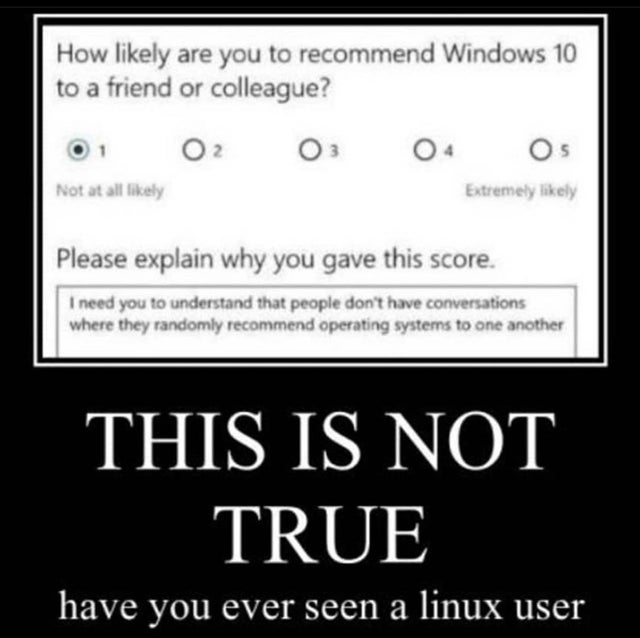
\includegraphics[width=.6\textwidth]{images/linux-user.jpg}
\end{center}


\end{frame}


\begin{frame}
\frametitle{Introduction to Operating Systems}

An operating system (OS) sits between the hardware and programs.

It has many goals, that often conflict with one another.

Its job is to make it so other programs can run efficiently.

\end{frame}

\begin{frame}
\frametitle{Structural Diagram of a Modern Computer}

\begin{center}
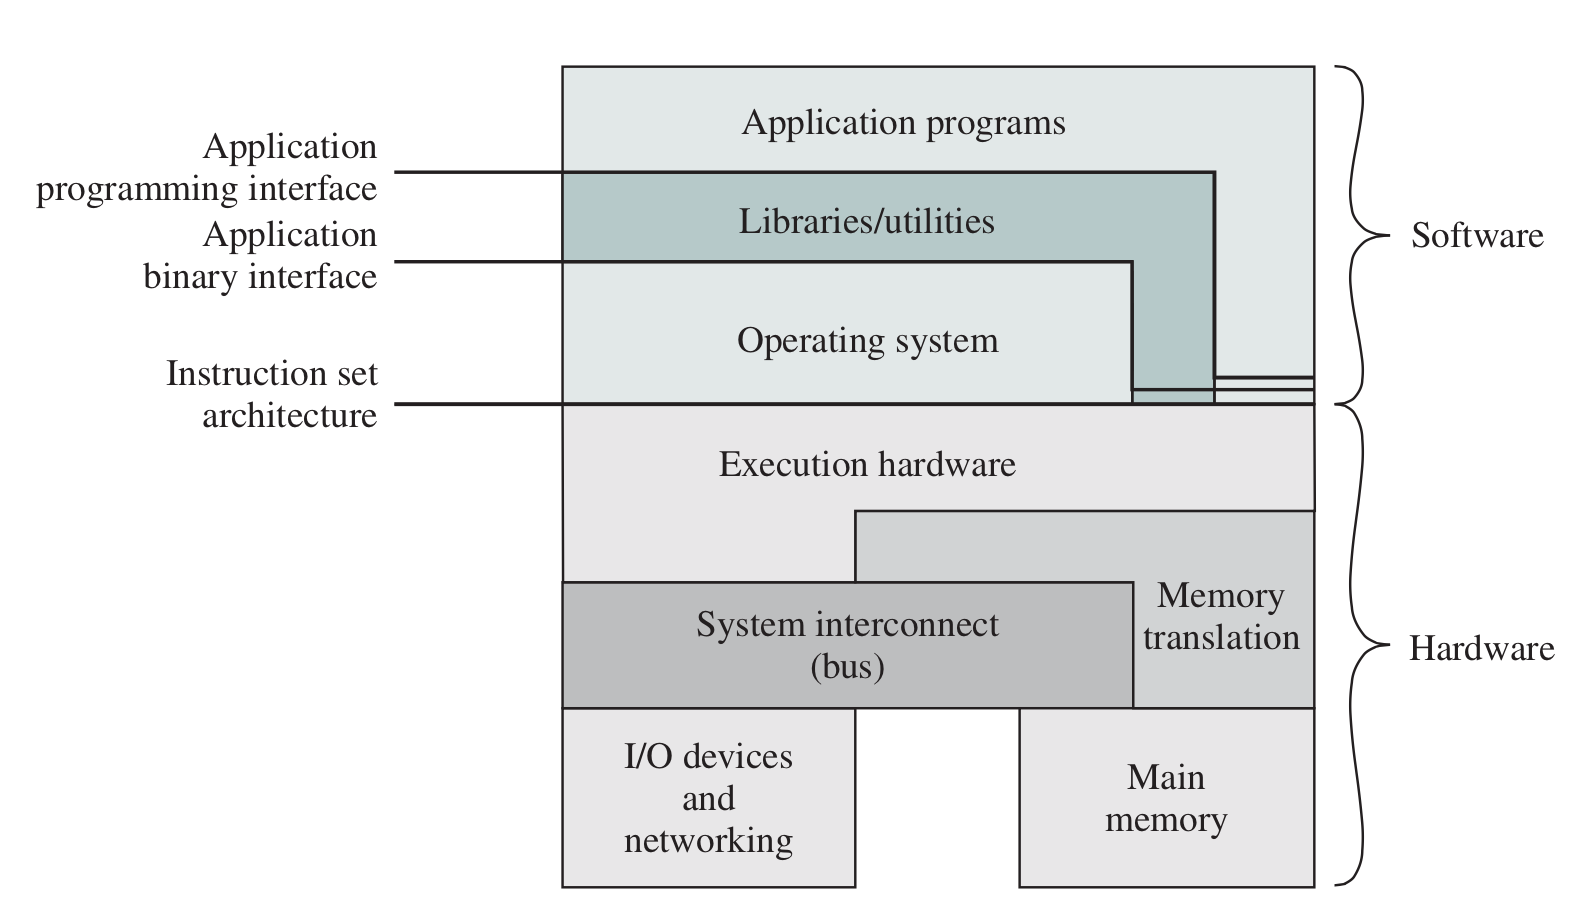
\includegraphics[width=0.95\textwidth]{images/os-sw-hw.png}
\end{center}

\end{frame}


\begin{frame}
\frametitle{OS: Resource Manager}

The OS is responsible for resource management and allocation.

Resources like CPU time or memory space are limited.

The OS must decide how to allocate \& to keep track of system resources.

In the event of conflicting requests, choose the winner.


\end{frame}

\begin{frame}
\frametitle{OS: Environment Provider}

The OS enables useful programs like Photoshop or Microsoft Word to run. 

The OS is responsible for abstracting away the details of hardware.

This is so program authors do not have to worry about the specifics.

Imagine Hello World had to be written differently for different hardware.


\end{frame}

\begin{frame}
\frametitle{OS: Multitasking}
Multiple programs means some resources are shared.\\
\quad $\rightarrow$ A source of conflicts!

OS creates and enforces the rules so all can get along.

\begin{center}
	
\includegraphics[width=0.4\textwidth]{images/sharing-is-caring.jpg}
\end{center}

Sometimes processes want to co-operate and not compete.\\
\quad The OS can help them to do so.


\end{frame}

\begin{frame}
\frametitle{OS: Efficiency}
Another goal may be to use the computer hardware efficiently.

\begin{center}
	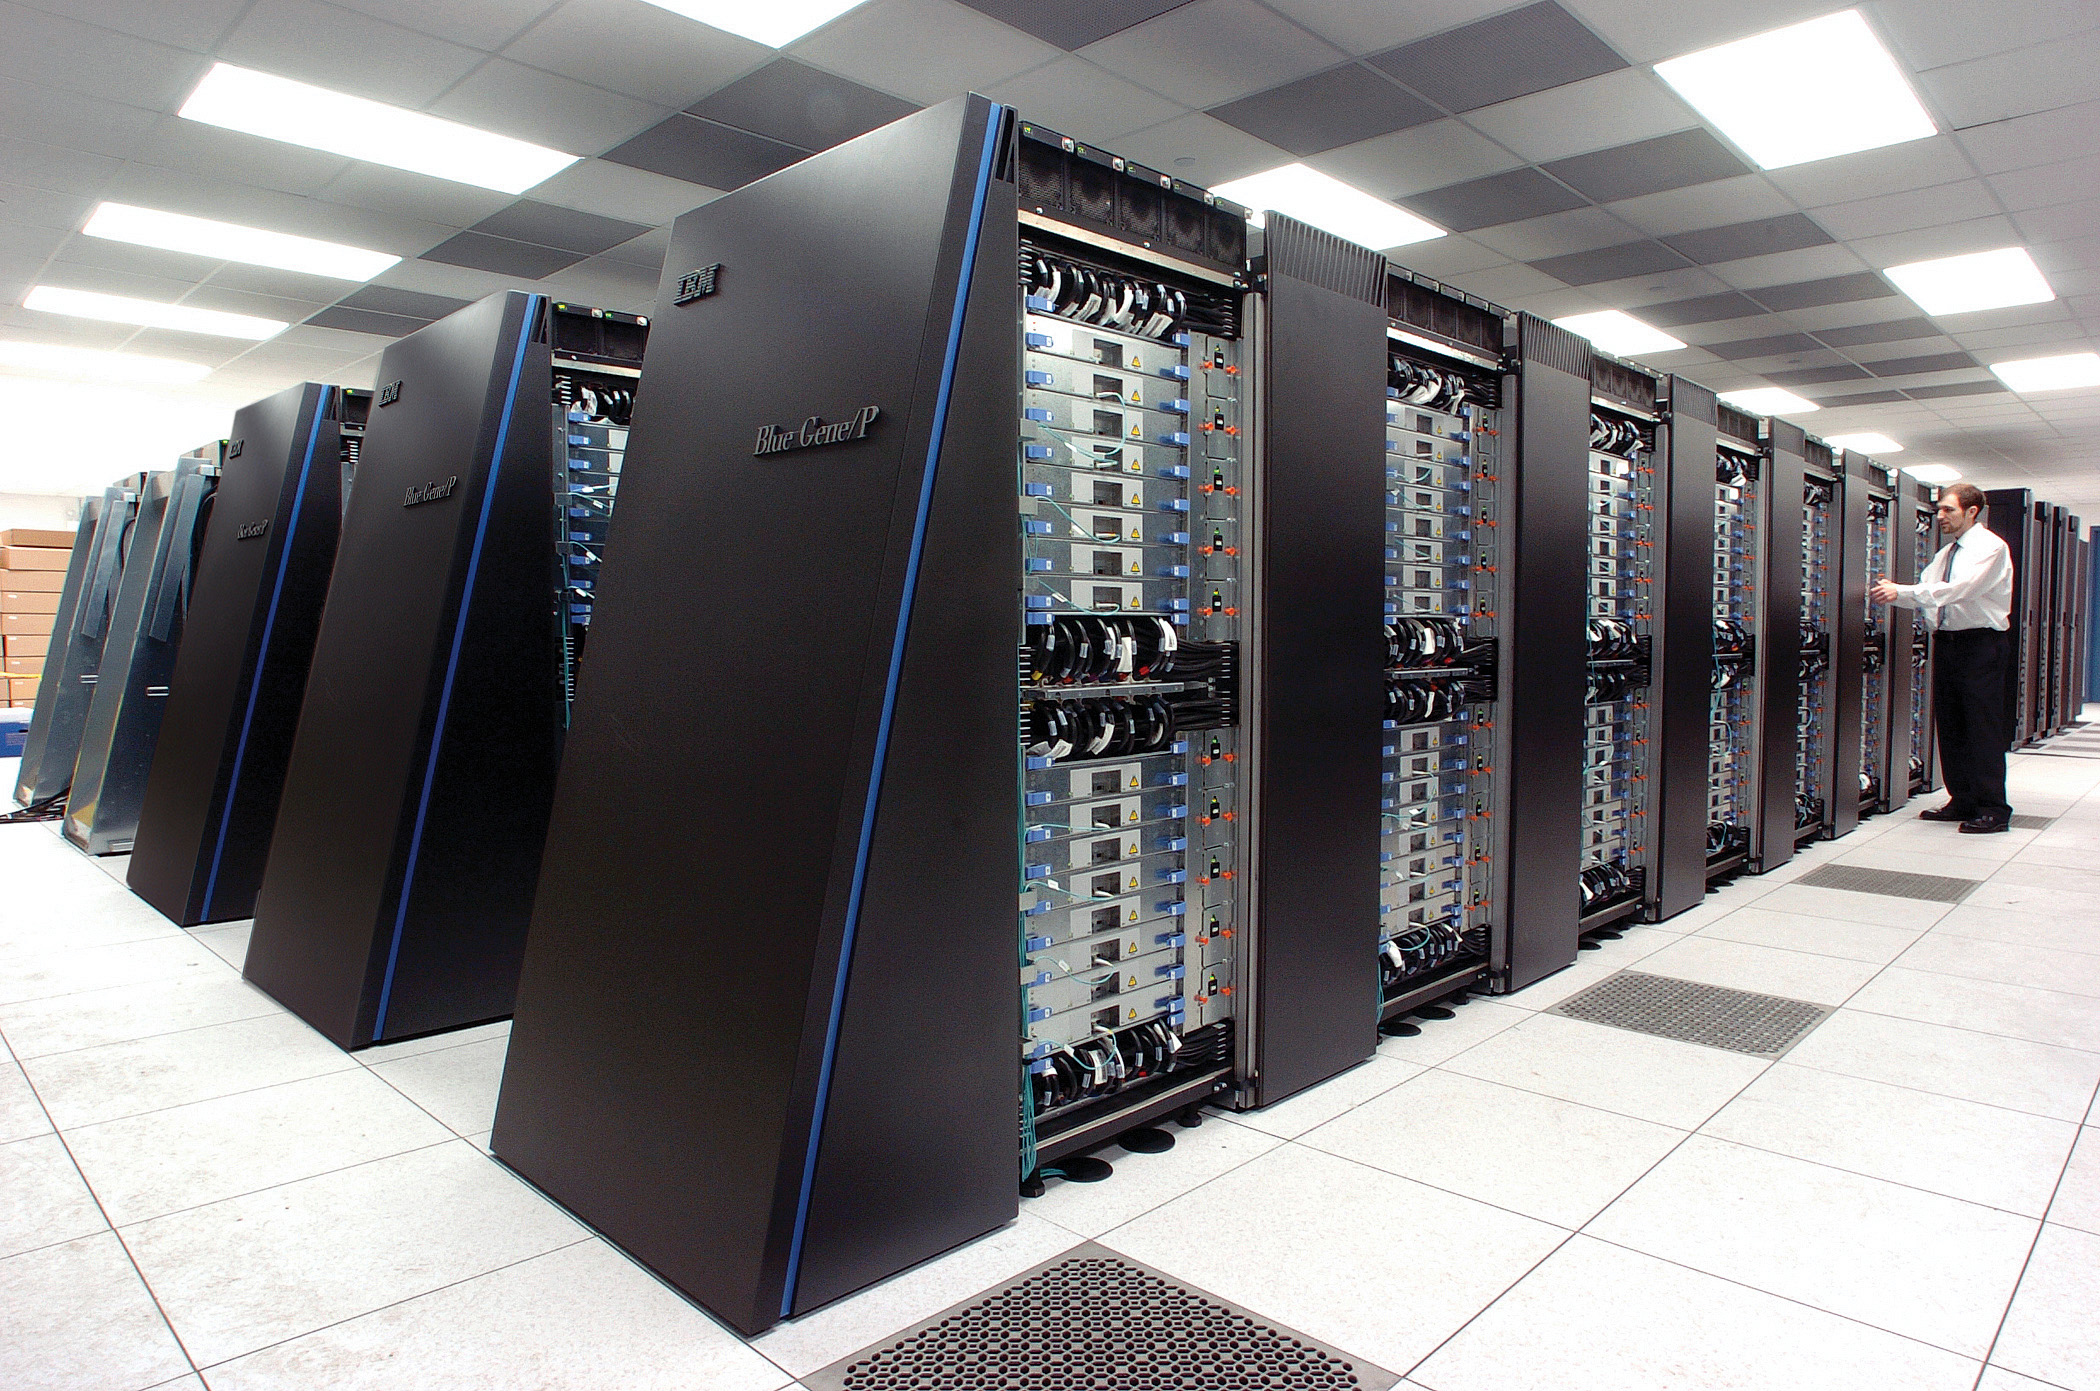
\includegraphics[width=0.7\textwidth]{images/supercomputer.jpg}
\end{center}
\hfill Image Credit: Argonne National Laboratory

Any moment when the supercomputer is not doing useful work is a waste.

\end{frame}

\begin{frame}
\frametitle{OS: What is it, really?}

Operating systems tend to be large and do a lot of things. 

We expect now that an OS comes with a web browser, an e-mail client, some method for editing text, et cetera. 

The part of the operating system we will study is the \alert{Kernel}.

The kernel is the ``core''; the portion of the OS that is always present in main memory and the central part that makes it all work.

\end{frame}

\begin{frame}
\frametitle{OS: Evolution}
Operating systems will evolve over time. 

There will be new hardware released, new types of hardware, new services added, and bug fixes. 

Evolution is constrained: a need to maintain compatibility for programs. 

\begin{center}
	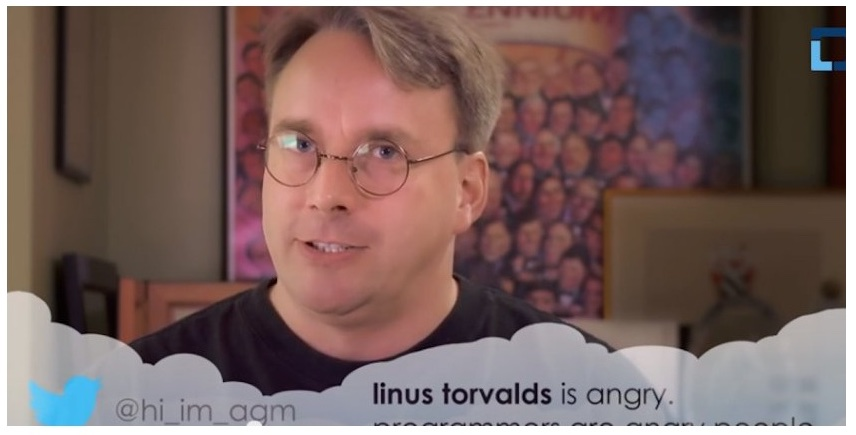
\includegraphics[width=0.7\textwidth]{images/linus-angry.jpg}
\end{center}

\end{frame}


\begin{frame}
\frametitle{Example: SimCity and Windows 95}

\begin{center}
	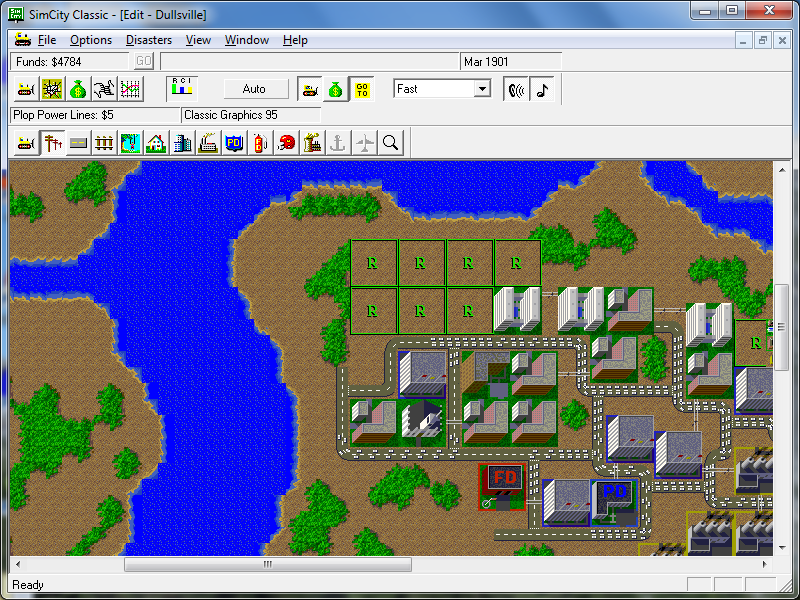
\includegraphics[width=0.85\textwidth]{images/simcity.png}
\end{center}

\end{frame}



\begin{frame}
\frametitle{Security Now}

\begin{center}
	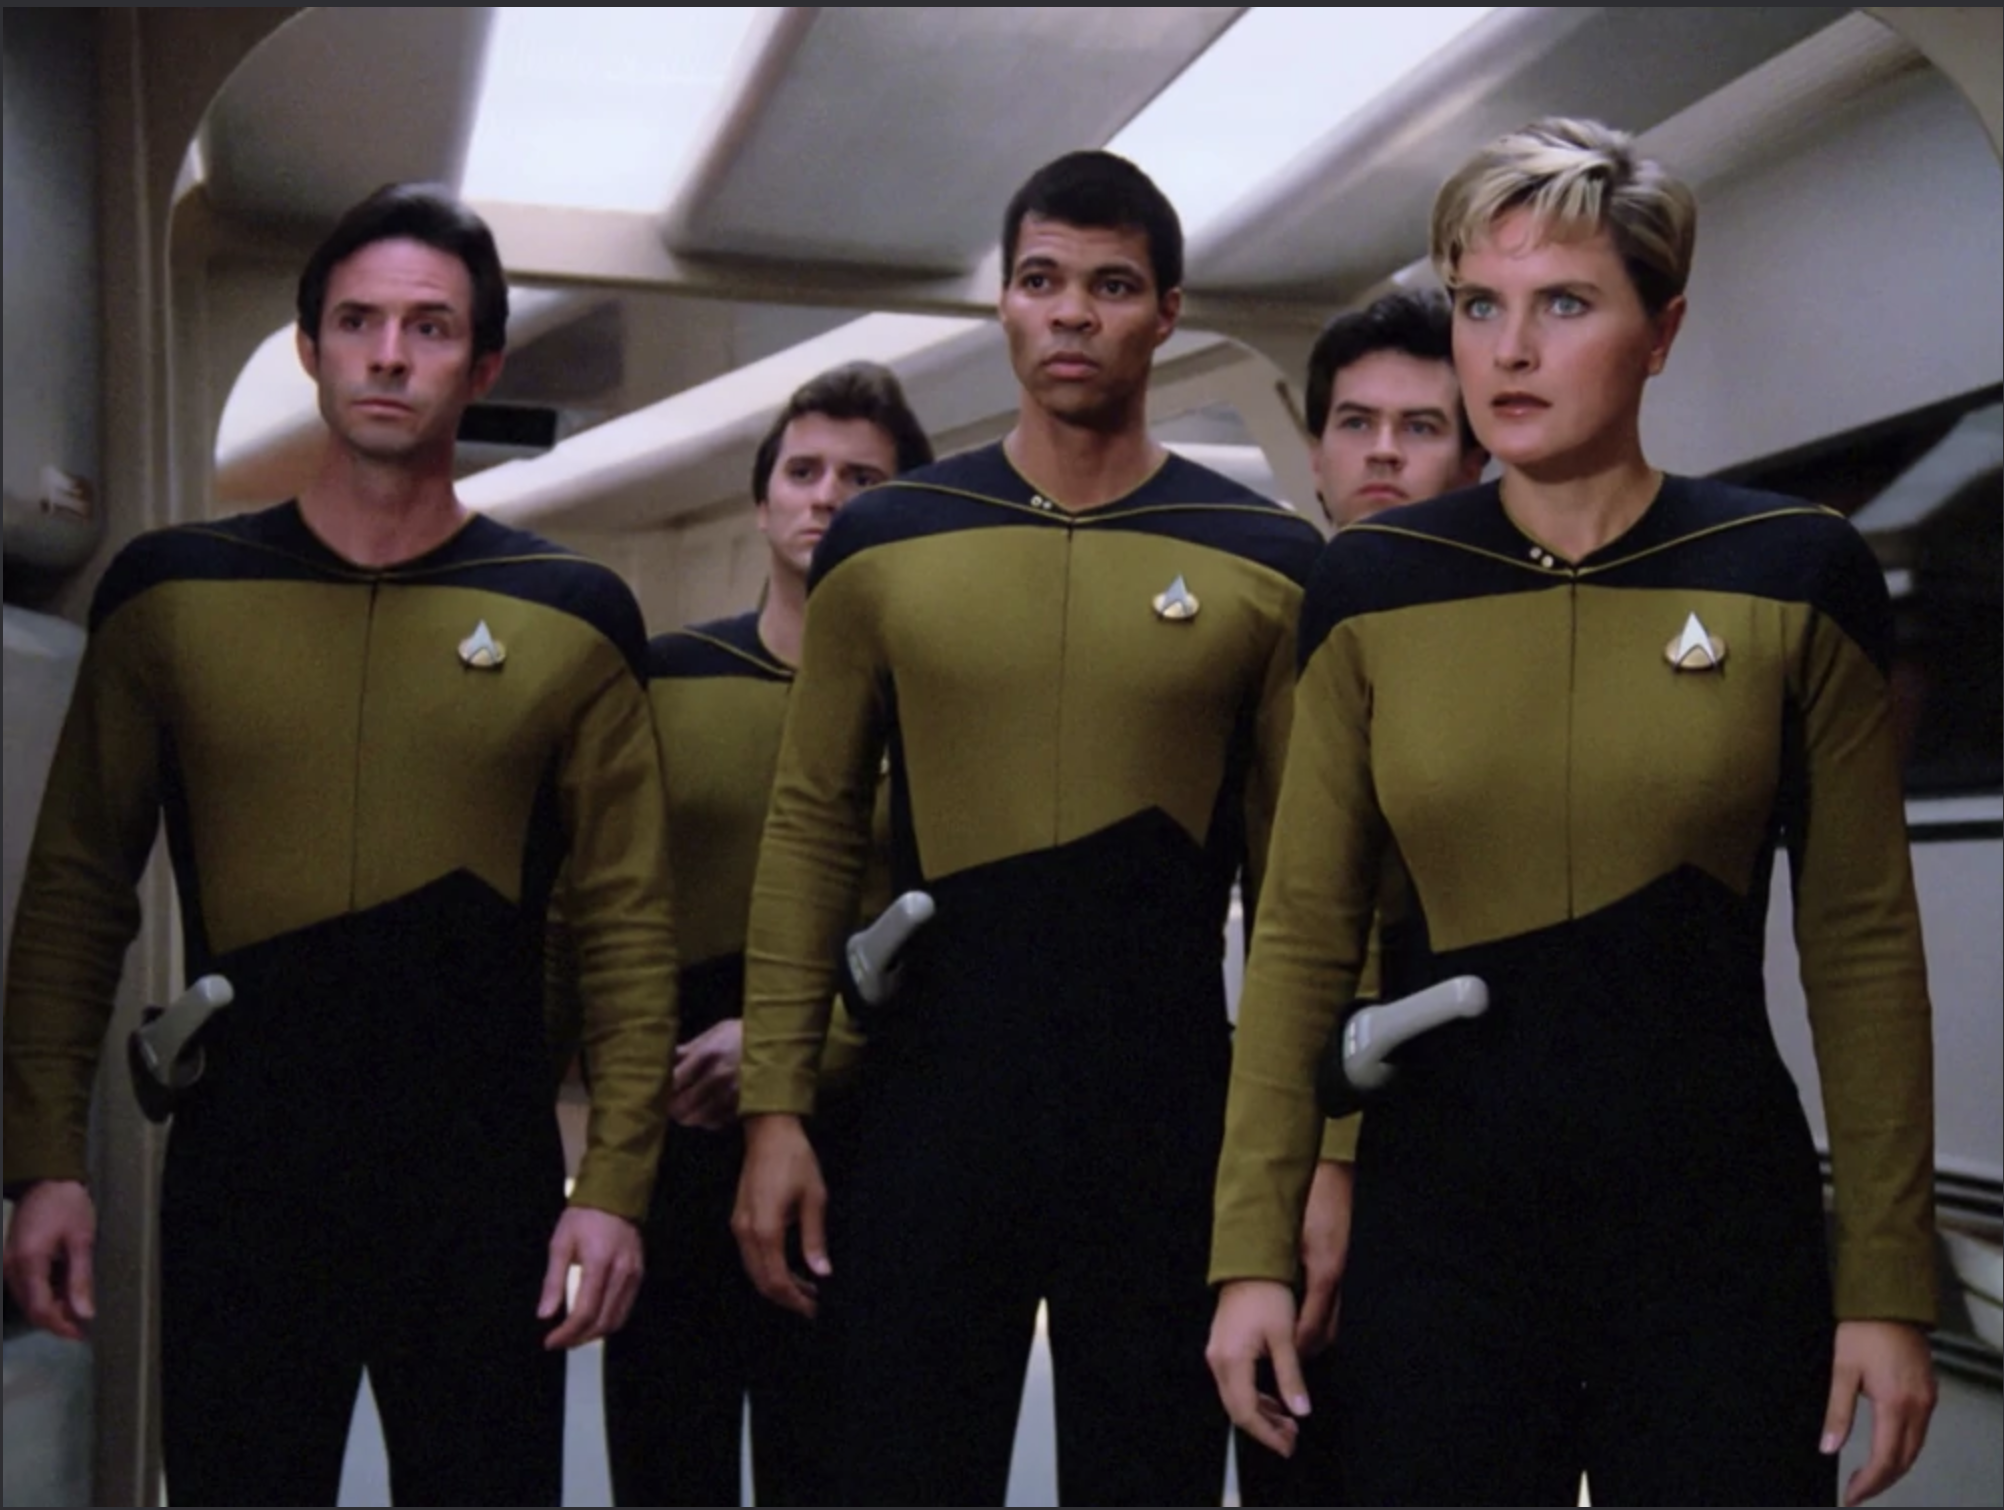
\includegraphics[width=0.9\textwidth]{images/security-team.png}
\end{center}


\end{frame}


\begin{frame}
\frametitle{Security Now}

In many textbooks, security and protection are left to the end.

Security has to be designed from the beginning; cannot be bolted on.

An OS supports multiple users with multiple tasks.

\end{frame}


\begin{frame}
\frametitle{Tool Support}

OS designers create policies and policy tools.

There is a tradeoff with usability.

You do NOT want to have to report a data breach.

\begin{center}
	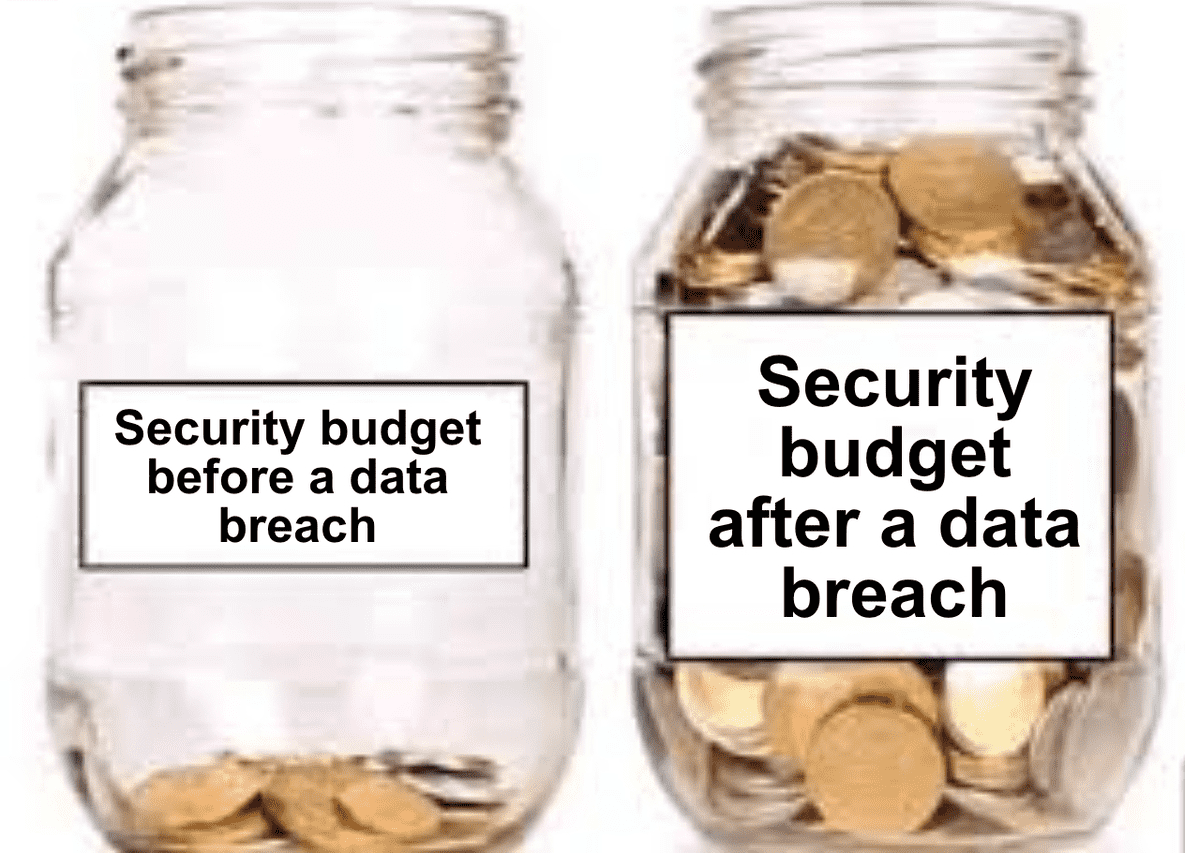
\includegraphics[width=0.35\textwidth]{images/security-budget.png}
\end{center}


\end{frame}


\begin{frame}
\frametitle{Enforcement is Everything}

The OS must enforce the configured policies.\\
\quad Otherwise, malicious users exploit it.

Three desirable properties: Confidentiality, Integrity, Availability.

\end{frame}


\begin{frame}
\frametitle{Protection vs Security}

Protection is about internal threats.

Security is about external threats.

We'll take them in order.


\end{frame}


\begin{frame}
\frametitle{Protection}

\begin{center}
	\includegraphics[width=\textwidth]{images/protection.jpg}
\end{center}


\end{frame}

\begin{frame}
\frametitle{Protection}

Most of the discussion in this course is about protection.

Following the rules is important to a functioning system or society.

Even in the absence of malicious intent.


\end{frame}


\begin{frame}
\frametitle{Goals of Protection}

Enforce policies about responsible usage.

Responsible and reasonable vary across systems.

Examples of access control: file permissions, walls between processes.

\end{frame}


\begin{frame}
\frametitle{Enforcement is Key}

Rules take effort to enforce.

Exceptions are allowed and administrators can override policies!

\begin{center}
	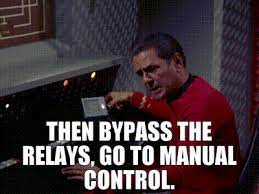
\includegraphics[width=0.4\textwidth]{images/override.jpg}
\end{center}

Other kinds of rules can exist.

\end{frame}


\begin{frame}
\frametitle{Context is Key}

If I edit a lecture video, it consumes a lot of CPU and RAM.

Is that bad?

It's legitimate -- but might set off alarms.

So we may be lax -- which gives an opening to malicious users...


\end{frame}



\begin{frame}
\frametitle{Security}

\begin{center}
	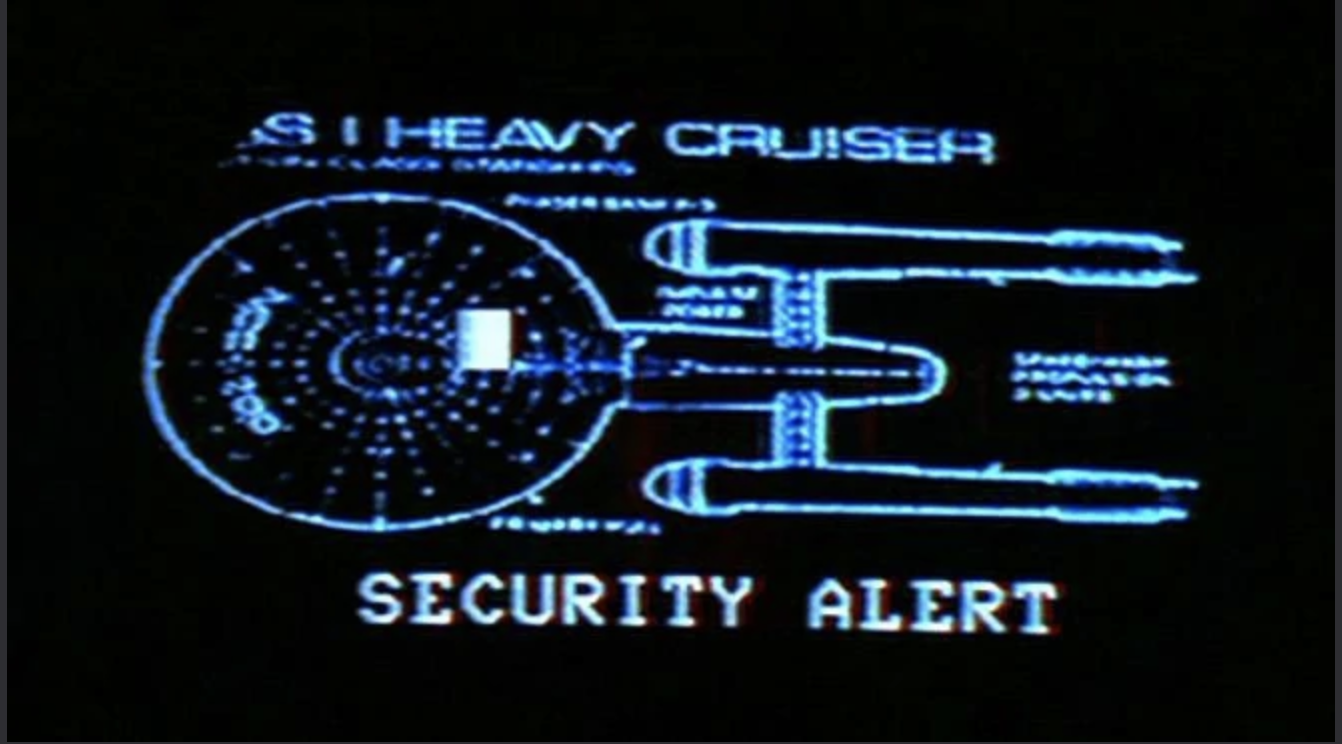
\includegraphics[width=0.4\textwidth]{images/security-alert.png}
\end{center}

Let's consider a few bad things attackers can do.

Why? We need this in mind when designing the system.


\end{frame}


\begin{frame}
\frametitle{Security Problems}

\begin{itemize}
	\item Breach of Confidentiality
	\item Breach of Integrity
	\item Breach of Availability
	\item Theft of Service
	\item ... and others.
\end{itemize}

Most likely the weak link is people.

\end{frame}


\begin{frame}
\frametitle{Specific Attacks}
A few potential specific attacks:

\begin{itemize}
	\item \textbf{Excessive Requests}
	\item \textbf{Malformed Requests}
	\item \textbf{Back Door}
	\item \textbf{Intercepting Messages}
	\item \textbf{Trojan Horse}
\end{itemize}


\end{frame}


\begin{frame}
\frametitle{Arms Race}

Security is an arms race.

Can we break things if it's a security problem?

No easy answers.


\end{frame}


\begin{frame}
\frametitle{Security, Conclusion}

This is not a course in security, but we can't ignore it.

Security needs to be included from the beginning!


\end{frame}


\begin{frame}
\frametitle{The Plan}

A broad overview of the major topics of the course:

\begin{enumerate}
	\item Introduction, Security, Review of Architecture
	\item Processes, Inter-Process Communication
	\item Threads, Concurrency,Synchronization, Deadlock
	\item Memory
	\item Scheduling
	\item I/O Devices, File Systems
\end{enumerate}

\end{frame}



\end{document}

